\section{System Overview}
\label{sec:system_overview}

This section presents a comprehensive overview of the collaborative dual-arm robotic brick assembly system. The architecture is designed hierarchically with five distinct layers, each with specific responsibilities and interactions. Figure~\ref{fig:system_architecture} illustrates the complete system architecture, demonstrating the top-down control flow from user input through hardware execution.
\begin{figure}[H]
    \centering
    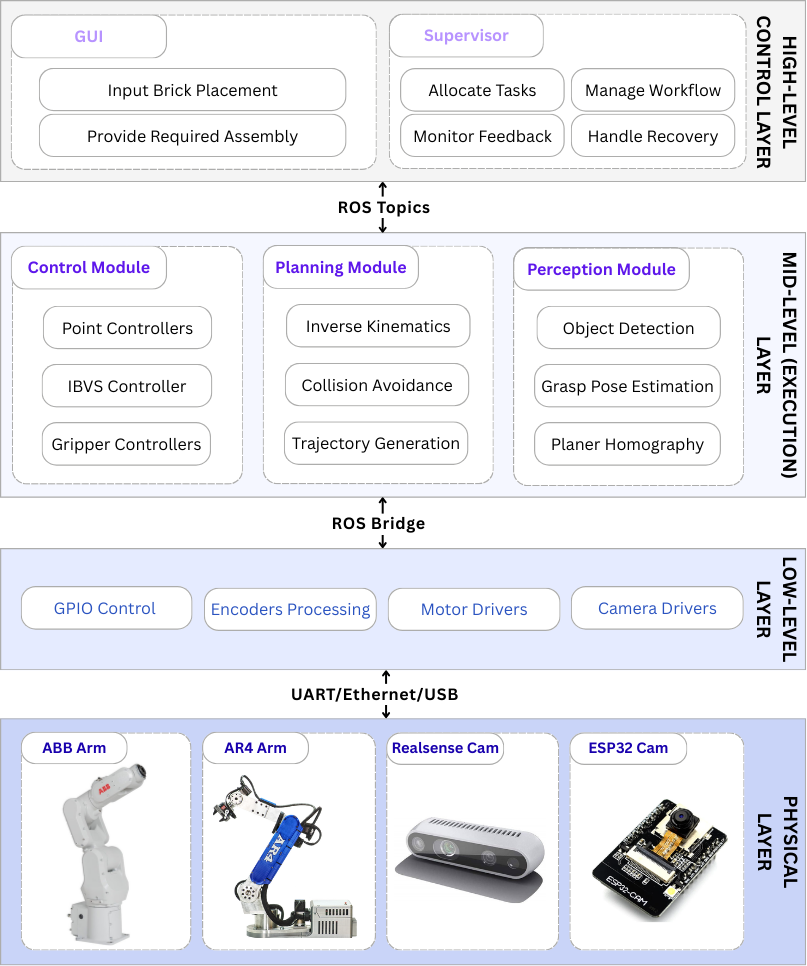
\includegraphics[width=0.73\textwidth]{Figures/chapter3/System_architecture/Architecture.png} 
    \caption{System Main Layers.}
    \label{fig:system_architecture}
\end{figure}

\subsection{System Architecture Overview}
\label{subsec:architecture_overview}

The system follows a layered architecture pattern, which enables modularity, maintainability, and clear separation of concerns. The architecture consists of five primary layers:

\begin{enumerate}
    \item \textbf{High-Level User Interface (GUI) Layer}: User interaction and task specification
    \item \textbf{Supervisor Layer}: Task allocation, workflow management, and synchronization
    \item \textbf{Mid-Level Execution (ROS) Layer}: Control, planning, and perception modules
    \item \textbf{Low-Level Hardware Abstraction Layer}: Driver abstraction and hardware communication
    \item \textbf{Physical Hardware Layer}: Robotic arms, grippers, cameras, and embedded systems
\end{enumerate}

Each layer abstracts the complexity of lower layers and provides a well-defined interface to higher layers, facilitating independent development and testing of components.

\subsection{Layer 1: High-Level User Interface (GUI) Layer}
\label{subsec:gui_layer}

\subsubsection{Overview and Purpose}
The GUI layer serves as the primary interface for specifying desired brick assembly configurations, it is used exclusively to define the target assembly pattern that the system should achieve. The GUI is the entry point for task specification and enables operators to intuitively construct complex brick arrangements without low-level programming.

\subsubsection{Key Components}

\textbf{Grid-Based Assembly Editor}: The GUI provides a grid-based interface where operators place bricks in desired positions (rows and columns) to define the target assembly. The interface supports:
\begin{itemize}
    \item \textbf{Four Brick Types}: Selection from a library of distinct brick geometries
    \item \textbf{Rotational Control}: Each brick can be rotated in four main angles (0°, 90°, 180°, 270°) to define orientation
    \item \textbf{Spatial Placement}: Drag-and-drop placement on a 2D grid representing the assembly workspace
    \item \textbf{Grid Coordinates}: Each position maps to specific row and column indices defining the target location
\end{itemize}

\textbf{Task Specification Output}: Once the user defines the desired arrangement, the GUI generates a structured task specification including:
\begin{itemize}
    \item Brick type for each grid position
    \item Rotation angle for each brick (0°, 90°, 180°, 270°)
    \item Row and column indices defining placement locations on the grid
\end{itemize}

This task specification is submitted to the Firestore database as a JSON document for persistent storage.

\subsubsection{Implementation Details}
The GUI is implemented as a web application that communicates with the robotic system through a cloud database backend. The architecture includes:

\begin{itemize}
    \item \textbf{Web Application Frontend}: A responsive web interface (JavaScript) that runs in a user's browser, providing the grid-based brick placement editor
    
    \item \textbf{Firestore Database Backend}: The GUI submits task specifications to a Google Firestore database in the following structure:
    \begin{itemize}
        \item JSON document containing the complete task specification
        \item Fields for each grid position: brick type and rotation angle
        \item Row and column indices
        \item Timestamp and task metadata for tracking
    \end{itemize}
    
    \item \textbf{ROS 2 Database Bridge with Assembly Allocator}: A dedicated ROS 2 Python node that serves as the critical interface between the GUI specification and robot execution. The node operates in two stages:
    
    \begin{enumerate}
        \item \textbf{Task Retrieval and Parsing}:
        \begin{itemize}
            \item Continuously monitors the Firestore database for new task submissions
            \item Fetches the JSON document using configured Firestore keys
            \item Extracts row/column indices, brick types, and rotations from the JSON
            \item Performs coordinate transformation from grid indices to desired 3D workspace coordinates using known grid spacing, brick dimensions, and workspace origin offset
        \end{itemize}
        
        \item \textbf{Assembly Allocator}:
        \begin{itemize}
            \item Subscribes to brick detections from the Perception Module (current brick positions in 3D workspace)
            \item Compares the desired arrangement (from GUI) against the available detected bricks in the current scene
            \item Validates that all required bricks are present and properly detected with sufficient confidence
            \item Performs spatial matching: associates each desired grid position with a detected brick instance
            \item Upon successful validation, generates an assembly plan containing:
            \begin{itemize}
                \item For each brick: current 3D position (XYZ) acquired from detection
                \item For each brick: desired 3D position (XYZ) computed from GUI specification
                \item Brick type and required rotation
            \end{itemize}
        \end{itemize}
    \end{enumerate}
    
    The assembly plan is published to the Supervisor, which then coordinates robot execution to move each brick from its current detected position to the desired position.
    
    
    \item \textbf{Decoupling Advantage}: By using Firestore as an intermediary, the GUI is completely decoupled from the ROS 2 system. The web application requires no ROS knowledge or configuration, and can be deployed independently on any web server. The database acts as a reliable, persistent message queue that survives temporary system disconnections.
    
    \item \textbf{No Real-Time Feedback}: The GUI remains purely an input specification tool; it receives no real-time feedback from the robot system
\end{itemize}

The Supervisor and Perception modules are responsible for determining the current state of the workspace and planning actions to achieve the GUI-specified configuration retrieved from the Firestore database.

\subsection{Layer 2: Supervisor Layer}
\label{subsec:supervisor_layer}

\subsubsection{Overview and Purpose}
The Supervisor layer represents the core orchestration component of the system. It manages the coordination between two independent robotic arms (ABB and AR4), handles workflow synchronization, monitors feedback from lower layers, and implements recovery mechanisms when anomalies occur. The Supervisor is responsible for translating high-level task specifications into concrete control commands for individual robots.

\subsubsection{Key Responsibilities}

\textbf{Assembly Plan Retrieval and Task Dequeuing}: The Supervisor retrieves the assembly plan from the ROS 2 Database Bridge node (via service call). This plan contains the ordered sequence of bricks to assemble, with both current and desired positions. The Supervisor maintains an assembly queue and dequeues bricks for processing.

\textbf{Perception Integration and Transform Management}: The Supervisor coordinates global brick detection from the RealSense camera:
\begin{itemize}
    \item Invokes the detection service to obtain brick poses in the camera's optical frame
    \item Applies coordinate frame transformations (TF2) to convert all detected brick poses to the ABB base frame
    \item Computes and transforms the handover pose (neutral zone between the two robots)
    \item Validates spatial consistency of all detected poses
\end{itemize}

\textbf{Grasp Planning and Selection}: For each brick to be grasped:
\begin{itemize}
    \item Queries the grasp inference service to obtain the optimal grasp candidate for the current brick
    \item Receives grasp pose (with quality metrics) in the camera frame
    \item Transforms grasp pose to the ABB base frame and applies safety constraints (e.g., minimum height clamps)
\end{itemize}

\textbf{Motion Execution and Robot Coordination}: The Supervisor issues concrete motion commands to both robots via action servers:
\begin{itemize}
    \item \textbf{AR4 Execution}: Submits point control actions for approach, grasp, and placement motions; optionally triggers visual servoing (IBVS) via the ESP32 wrist camera for precision control
    \item \textbf{ABB Execution}: Submits high-level task actions (pick, place, pick-from-handover) that are internally managed by the ABB controller
    \item \textbf{Handover Coordination}: If handover strategy is selected, orchestrates synchronized execution where AR4 picks a brick and ABB receives it at the handover pose
\end{itemize}

\textbf{Strategy Selection and Allocation Logic}: The Supervisor decides between two execution strategies:
\begin{itemize}
    \item \textbf{Direct Assembly}: Robot directly picks and places a brick when reachable and collision-free
    \item \textbf{Handover Strategy}: AR4 picks the brick and passes it to the ABB at the handover zone for placement, enabling access to areas unreachable by AR4 alone
\end{itemize}

\textbf{State Machine Management}: The Supervisor implements a multi-state finite state machine that coordinates the complete workflow:
\begin{itemize}
    \item INIT: Retrieve assembly plan from Database Bridge
    \item DETECT: Perform global brick detection and transform poses
    \item PROCESS\_NEXT: Dequeue next brick from assembly queue
    \item GRASP\_PIPELINE: Query grasp inference service for selected brick
    \item Execution States: EXECUTE\_AR4\_DIRECT, AR4\_PICK\_FOR\_HANDOVER, EXECUTE\_ABB\_PICK, EXECUTE\_ABB\_PLACE, HANDOVER\_EXECUTION
    \item DONE: Assembly complete; system idle
\end{itemize}

\textbf{Error Handling and Recovery}: When anomalies occur:
\begin{itemize}
    \item Detects service failures and timeouts
    \item Implements retry logic with controlled backoff
    \item Logs detailed error information for debugging
\end{itemize}

\subsubsection{Implementation Details}
The Supervisor is implemented as a ROS2 Python node that maintains continuous communication with all lower-layer modules. It uses ROS2 services for synchronous task initiation and topics for asynchronous feedback. Key implementation aspects include:

\begin{itemize}
    \item \textbf{Namespaced Robot Control}: Uses ROS 2 namespace hierarchies (\texttt{/abb/}, \texttt{/ar4/}) to maintain separate action clients and service clients for each robot, enabling independent command submission
        
    \item \textbf{Action-Based Synchronization}: Uses ROS 2 action servers for non-blocking, feedback-capable task execution. The Supervisor submits action goals and blocks until completion, ensuring tasks execute serially
    
    \item \textbf{Timing and Synchronization}: Implements timeout mechanisms and heartbeat monitoring to detect stalled or crashed components.
    
    \item \textbf{Multi-Threaded Executor}: Employs a reentrant callback group allowing concurrent handling of service requests and action goal submissions without blocking the main state machine loop
\end{itemize}

\subsection{Layer 3: Mid-Level Execution Layer (ROS Modules)}
\label{subsec:ros_layer}

The mid-level execution layer consists of three independent but interconnected ROS 2 modules: Control, Planning, and Perception. These modules implement the core algorithmic components of the system and directly interface with hardware through the abstraction layer below.

\subsubsection{3.1 Control Module}
\label{subsubsec:control_module}

\textbf{Overview}: The Control Module translates high-level motion objectives into low-level joint commands. It implements multiple control strategies tailored to different task phases and ensures robust execution despite environmental variations.

\textbf{Key Components}:

\begin{itemize}
    \item \textbf{Point Controllers}: Implemented as ROS 2 action servers that receive desired end-effector coordinates (Cartesian pose) from the Supervisor. The Point Controllers:
    \begin{itemize}
        \item Accept a goal containing target coordinates (X, Y, Z, orientation)
        \item Delegate motion planning and trajectory computation to MoveIt2
        \item Execute the planned trajectory on the physical robot via the Hardware Abstraction Layer
        \item Provide feedback on execution progress and result status
        \item Do not directly compute IK or trajectories; MoveIt2 handles all planning logic
    \end{itemize}
        
    \item \textbf{IBVS (Image-Based Visual Servoing) Controller}: For the AR4 arm, the IBVS controller provides visual feedback correction during pick-and-place operations. This is critical for:
    \begin{itemize}
        \item Compensating for small calibration errors
        \item Correcting for environmental variations (brick surface reflectivity, lighting)
        \item Fine-tuning gripper approach trajectories
        \item Providing closed-loop feedback during manipulation
    \end{itemize}
    
    The IBVS uses the ESP32 wrist-mounted camera as feedback and implements visual feature tracking (edges, corners) to maintain precise alignment with the target brick. The visual error is converted to velocity commands using the camera Jacobian.
    
    \item \textbf{Gripper Controllers}: Manage pneumatic (ABB) and servo-based (AR4) grippers with:
    \begin{itemize}
        \item Open/close state management
    \end{itemize}
\end{itemize}

\textbf{Implementation Details}:
The Control Module runs as separate ROS 2 action servers for each robot (one per arm). Each action server:
\begin{itemize}
    \item Receives motion goals (target coordinates) from the Supervisor
    \item Calls MoveIt2's planning and execution interfaces to compute and execute trajectories
    \item Monitors execution status and provides feedback to the Supervisor
    \item Publishes low-level joint commands at rates of 100-500 Hz depending on the control strategy
    \item Implements safety monitoring for joint limits, velocity limits, and collision detection
\end{itemize}

\subsubsection{3.2 Planning Module}
\label{subsubsec:planning_module}

\textbf{Overview}: The Planning Module computes collision-free trajectories and solves inverse kinematic problems. It serves as the interface between high-level task objectives and concrete motion commands, ensuring that all computed motions are feasible and safe.

\textbf{Key Components}:

\begin{itemize}
    \item \textbf{Inverse Kinematics (IK) Solvers}: Two solvers are employed with selective switching based on active control mode:
    \begin{itemize}
        \item \textbf{IKFast (Analytical Solver)}: The default solver for both AR4 and ABB arms. Provides fast, exact solutions by leveraging pre-computed closed-form solutions offline, enabling real-time IK queries with multiple solution branches
        \item \textbf{KDL (Numerical Solver)}: Used exclusively for AR4 when Image-Based Visual Servoing (IBVS) is active. The iterative numerical approach allows continuous refinement of joint configurations in response to visual feedback, which is essential for the precision correction that IBVS provides
        \item \textbf{Solver Switching Logic}: When IBVS is activated on AR4, the IK solver switches from IKFast to KDL to support real-time visual servo corrections. When IBVS is inactive, both robots use IKFast for rapid planning and execution
    \end{itemize}
        
    \item \textbf{Path Planning (RRTconnect)}: Uses MoveIt2's interface to OMPL (Open Motion Planning Library) with the RRTconnect algorithm as the primary motion planner. RRTconnect:
    \begin{itemize}
        \item Employs bi-directional Rapidly-Exploring Random Trees (RRT) from both start and goal configurations
        \item Grows two trees simultaneously, one from the start state and one from the goal state, significantly accelerating convergence
        \item Effective for high-dimensional configuration spaces, suitable for 6-DOF robotic arms
        \item Naturally handles complex environments with obstacles and narrow passages through randomized exploration
        \item Produces kinematically feasible paths without requiring analytical solutions
    \end{itemize}
    
    The path planner operates on a collision model that includes:
    \begin{itemize}
        \item Robot self-collision models (defined in URDF)
        \item Environment obstacles (static table, fixed structures)
        \item Other robot (for collision avoidance between arms)
    \end{itemize}
    
    \item \textbf{Collision Avoidance}: Beyond path planning, collision detection occurs at two levels:
    \begin{itemize}
        \item \textbf{Planning Phase}: OMPL checks collisions during trajectory sampling
        \item \textbf{Execution Phase}: Real-time collision detection using joint feedback validates that actual motion matches planned motion
    \end{itemize}
    
    \item \textbf{Trajectory Generation}: Converts paths (sequences of configurations) into time-parameterized trajectories respecting velocity and acceleration limits. MoveIt2 handles trajectory parameterization using:
    \begin{itemize}
        \item Time-optimal trajectory parameterization for efficient motion
        \item Joint velocity and acceleration limits configured per robot 
        \item Gripper-specific constraints 
    \end{itemize}
\end{itemize}

\textbf{Implementation Details}:
The Planning Module is implemented as a ROS2 C++ node with direct MoveIt2 integration. MoveIt2 encapsulates RRTconnect planning, IK solving, and trajectory parameterization. Key architectural aspects:

\begin{itemize}
    \item \textbf{Asynchronous Planning}: Planning requests are handled asynchronously to avoid blocking the Supervisor
    \item \textbf{Planning Scene Updates}: Maintains a collision world model that is continuously updated with:
    \begin{itemize}
        \item Detected object positions from the Perception Module
        \item Current robot states (to detect collisions in progress)
        \item Manual environment updates from the GUI
    \end{itemize}
    \item \textbf{Solver Selection Logic}: AR4 dynamically switches between IKFast (default) and KDL (when IBVS is active) based on control mode:
    \begin{itemize}
        \item \textbf{Standard Execution}: Both AR4 and ABB use IKFast for rapid, deterministic inverse kinematics
        \item \textbf{Visual Servo Active}: AR4 switches to KDL to enable continuous refinement guided by visual feedback from the ESP32 wrist camera. KDL's iterative nature allows online adjustment of joint configurations in response to perceived visual errors, whereas IKFast's pre-computed solutions are optimized for bulk solution generation rather than online refinement
    \end{itemize}
\end{itemize}

\subsubsection{3.3 Perception Module}
\label{subsubsec:perception_module}

\textbf{Overview}: The Perception Module processes visual data from the RealSense camera to understand the environment, detect objects, estimate grasp points, and provide visual feedback. It serves as the sensory foundation for autonomous decision-making throughout the system.

\textbf{Key Components}:

\begin{itemize}
    \item \textbf{Object Detection (YOLOv8 Segmentation)}: Uses YOLOv8 segmentation model to:
    \begin{itemize}
        \item Detect brick instances in the scene
        \item Provide pixel-level segmentation masks
        \item Output: Bounding boxes, class labels, confidence scores, and segmentation masks
        
        \item \textbf{Metrics}: Performance is evaluated using mean Average Precision (mAP) and Intersection over Union (IoU)
        \begin{itemize}
            \item mAP: Evaluates detection quality across all confidence thresholds
            \item IoU: Measures segmentation mask accuracy
        \end{itemize}
    \end{itemize}
    
    The YOLOv8 model is deployed with the Realsense scene camera (top-down view) to maintain a global view of brick locations and availability.
    
    \item \textbf{Grasp Point Generation (Transformer-Based Learning)}: Estimates optimal gripper approach poses for detected bricks. The system employs:
    \begin{itemize}
        \item \textbf{Vision Transformer (ViT) Architecture}: Encodes multi-scale image features to understand local geometric properties
        \item \textbf{Grasp Quality Estimation}: Learns to predict grasp success probability
        \item \textbf{4-DOF Pose Prediction}: Estimates gripper orientation and position relative to the brick
    \end{itemize}
    
    Grasp learning is trained on:
    \begin{itemize}
        \item Synthetic grasping datasets (procedurally generated)
        \item Real-world grasp attempts (labeled for success/failure)
    \end{itemize}
    
    The output is a grasping point with the highest confidence.
    \item \textbf{Grasp Pose Estimation}: Converts predicted gripper poses (relative to camera frame) into world coordinates:
    \begin{itemize}
        \item Camera calibration: Intrinsic parameters determined offline
        \item Camera-to-base transformation: Computed from known camera mounting geometry
        \item Coordinate transformation pipeline: RGB image → camera frame → robot base frame
    \end{itemize}
   
\end{itemize}

\textbf{Implementation Details}:
The Perception Module is implemented as a ROS 2 Python node with GPU-accelerated inference:

\begin{itemize}
    \item \textbf{Camera Feed Source}: Subscribes exclusively to:
    \begin{itemize}
        \item Realsense scene camera feed (for full YOLOv8 + grasp inference processing)
    \end{itemize}
        
    \item \textbf{Inference Pipeline}: 
    \begin{enumerate}
        \item Receive RGB frame from Realsense camera
        \item Preprocess: Resize, normalize to YOLOv8 input format
        \item Run YOLOv8 segmentation inference (GPU)
        \item For each detected brick: Extract ROI, run grasp transformer
        \item Convert output to world frame using calibrated transformations
        \item Publish detected objects and grasp candidates
    \end{enumerate}
    
    \item \textbf{Latency Optimization}: 
    \begin{itemize}
        \item Batched inference when multiple detections occur
        \item Asynchronous inference using thread pools to avoid blocking the main ROS loop
        \item Frame skipping for non-critical grasp updates
    \end{itemize}

\end{itemize}

\subsection{Layer 4: Low-Level Hardware Abstraction Layer}
\label{subsec:hardware_abstraction_layer}

\subsubsection{Overview and Purpose}
The Hardware Abstraction Layer (HAL) decouples high-level ROS modules from hardware-specific communication details. It provides standardized interfaces for hardware control and feedback, enabling seamless swapping of hardware implementations without changes to higher layers.

\subsubsection{Key Components}

\textbf{Encoder Processing}: Reads joint angle feedback from:
\begin{itemize}
    \item Robot joint encoders (via proprietary robot communication protocols)
\end{itemize}
\clearpage

\textbf{Motor Drivers}: Interface with:
\begin{itemize}
    \item AR4 servo motors (for joints and gripper)
    \item Motor control boards managing PWM signals 
\end{itemize}

\textbf{Camera Drivers}: ROS camera interface nodes for:
\begin{itemize}
    \item Realsense SDK integration (color, depth, point clouds)
    \item ESP32 camera module 
\end{itemize}

\textbf{Communication Protocols}: Manages hardware communication over:
\begin{itemize}
    \item UART/Serial (AR4 Communication)
    \item Ethernet (ABB Communication)
    \item USB (Camera Interfaces)
\end{itemize}

\subsubsection{Implementation Details}

The HAL is implemented as a set of specialized ROS2 nodes:

\begin{itemize}
    \item \textbf{Robot Driver Nodes}: Each robot (ABB, AR4) has a dedicated driver node that:
    \begin{itemize}
        \item Communicates with the robot controller using vendor-specific APIs
        \item Translates ROS command messages to robot commands
        \item Publishes robot state (joint positions, velocities, forces) on standardized ROS topics
        \item Implements hardware safety checks (joint limits, fault detection)
    \end{itemize}
    
    \item \textbf{Camera Driver Nodes}: 
    \begin{itemize}
        \item Realsense driver: Publishes RGB/Depth at configurable rates
        \item ESP32 driver: Custom firmware and ROS bridge for low-latency video streaming
    \end{itemize}
    
    \item \textbf{Standardized Topic Interfaces}: All hardware communication is abstracted to standard ROS2 topics:
    \begin{itemize}
        \item \texttt{/robot\_name/joint\_states}: Joint feedback
        \item \texttt{/robot\_name/command/joint\_trajectory}: Trajectory commands
        \item \texttt{/gripper/state}: Gripper status
        \item \texttt{/camera/rgb/image\_raw}: Camera feeds
    \end{itemize}
\end{itemize}

\subsection{Layer 5: Physical Hardware Layer}
\label{subsec:physical_hardware_layer}

\subsubsection{Overview}
The Physical Hardware Layer comprises the actual robotic systems, sensors, and actuators that interact with the physical world.

\subsubsection{Key Hardware Components}

\textbf{ABB Robotic Arm}: Industrial 6-DOF collaborative arm with:
\begin{itemize}
    \item High payload capacity
    \item Precise joint control via proprietary controller
    \item Pneumatic end-effector gripper for power grasping
\end{itemize}

\textbf{AR4 Robotic Arm}: Custom 6-DOF robotic arm with:
\begin{itemize}
    \item Servo-based joints (high precision, lower payload)
    \item Modular servo-gripper
    \item ESP32 wrist-mounted camera for close-range visual servoing
    \item Lighter weight, suitable for fine manipulation tasks
\end{itemize}

\textbf{Realsense Scene Camera}: Intel Realsense D435i camera:
\begin{itemize}
    \item Mounted at top of workspace, looking down
    \item Provides color image for YOLOv8 detection
\end{itemize}

\textbf{ESP32 Wrist Camera}: Customized lightweight camera module mounted on AR4 wrist:
\begin{itemize}
    \item OV2640 Wide angle lense 2MP camera sensor
    \item Real-time video streaming via WiFi
    \item Low power consumption (suitable for wrist mounting)
    \item Used exclusively for IBVS feedback 
\end{itemize}

\textbf{Gripper Hardware}:
\begin{itemize}
    \item ABB gripper: Pneumatic dual-finger, open/close control
    \item AR4 gripper: Servo-driven with force feedback and state feedback
\end{itemize}

\subsection{Cross-Layer Communication and Data Flow}
\label{subsec:cross_layer_communication}

To complete the architectural understanding, this section describes how data and commands flow through the layered system:

\subsubsection{Top-Down Command Flow}
\begin{enumerate}
    \item \textbf{User Input}: Operator specifies a brick placing task in the GUI
    \item \textbf{Supervisor Interpretation}: Supervisor decomposes task into concrete motion commands
    \item \textbf{Planning}: Planning Module computes collision-free trajectories using IK and OMPL solvers
    \item \textbf{Control}: Control Module executes trajectories
    \item \textbf{Hardware Execution}: Motors and grippers execute commands, generating motion
\end{enumerate}

\subsubsection{Bottom-Up Feedback Flow}
\begin{enumerate}
    \item \textbf{Sensor Readings}: Hardware layer generates continuous sensor data (camera frames)
    \item \textbf{Hardware Abstraction}: HAL layer processes raw sensor data and publishes standardized ROS messages
    \item \textbf{Control Feedback}: Control Module uses feedback for closed-loop corrections (e.g., IBVS visual servo)
    \item \textbf{Perception Updates}: Perception Module processes camera data to update world state
    \item \textbf{Supervisor Monitoring}: Supervisor tracks task progress and detects anomalies
\end{enumerate}

\subsubsection{Lateral Communication}
Between-module communication enables coordination:
\begin{itemize}
    \item \textbf{Planning $\leftrightarrow$ Perception}: Planning Module queries Perception Module for current object poses
    \item \textbf{Control $\leftrightarrow$ Perception}: Control Module requests precision updates from Perception during delicate operations
    \item \textbf{Supervisor $\leftrightarrow$ All Modules}: Supervisor broadcasts state information and receives status updates from all lower layers
\end{itemize}

\subsection{Synchronization and Timing}
\label{subsec:synchronization_timing}

Proper timing synchronization is critical for multi-robot coordination. The system employs:

\begin{itemize}
    \item \textbf{ROS 2 Clock}: All nodes synchronized to ROS global clock (allows simulation time in Gazebo Harmonic)
    \item \textbf{Action Servers}: Asynchronous action servers ensure non-blocking execution of long-duration operations (trajectories, planning)
    \item \textbf{Watchdog Timers}: Detect stalled or crashed nodes through timeout mechanisms
\end{itemize}

\subsection{Simulation Environment}
\label{subsec:simulation_environment}

The system is developed and tested using Gazebo Harmonic, a high-fidelity physics simulator:

\begin{itemize}
    \item \textbf{Development Benefits}:
    \begin{itemize}
        \item Test algorithms without risking hardware damage
        \item Rapid prototyping and iteration
        \item Deterministic simulation for algorithm validation
    \end{itemize}
\end{itemize}

\subsection{System Properties and Design Considerations}
\label{subsec:system_properties}

\subsubsection{Modularity and Extensibility}
The layered architecture enables:
\begin{itemize}
    \item Independent development of each layer
    \item Swapping components (e.g., alternative planners, different gripper hardware) without system-wide refactoring
    \item Easy addition of new modules (e.g., force/torque feedback, additional sensors)
\end{itemize}

\subsubsection{Robustness and Fault Tolerance}
\begin{itemize}
    \item \textbf{Graceful Degradation}: Loss of one capability triggers fallback strategies
    \item \textbf{Multi-Modal Control}: IBVS + Point Control provides redundancy
    \item \textbf{Recovery Logic}: Supervisor detects and recovers from common failures
\end{itemize}

\subsubsection{Safety}
\begin{itemize}
    \item \textbf{Collision Detection}: Multiple layers check for collisions
    \item \textbf{Joint Limits}: All control layers respect hardware limits
\end{itemize}

